\documentclass[10pt]{beamer}

\usetheme[progressbar=frametitle]{metropolis}
\usepackage{appendixnumberbeamer}


\usepackage{array,booktabs}
\usepackage[scale=2]{ccicons}
\usepackage{multicol}
\usepackage{mathtools}
\usepackage{array}

\usepackage{pgfplots}
\usepgfplotslibrary{dateplot}

\usepackage{xspace}
\newcommand{\themename}{\textbf{\textsc{metropolis}}\xspace}
\let\oldfootnotesize\footnotesize
\renewcommand*{\footnotesize}{\oldfootnotesize\tiny}
\let\oldabs\abs
\def\abs{\@ifstar{\oldabs}{\oldabs*}}


\title{Lancaster A at SemEval-2017 Task 5: Evaluation metrics matter: predicting sentiment from financial news headlines}
\author{Andrew Moore and Paul Rayson}
\date{\today}
\institute{School of Computing and Communications, Lancaster University.}
\titlegraphic{\hfill
\includegraphics[height=1.5cm]{ucrel_logo_2016.png}}

\begin{document}

\maketitle

\section{Task}


\begin{frame}[fragile]{The task}
\begin{block}{Example sentence}
\begin{center}
`Why \alert{AstraZeneca plc} \& \alert{Dixons Carphone PLC} Are Red-Hot Growth Stars!'
\end{center}
\end{block}

\begin{block}{Sentiment scale}
\begin{figure}
    
\includegraphics[scale=0.3]{sentiment_range.png}
  \end{figure}
\end{block}

\begin{block}{Data}
Training data: 1142 samples, 960 headlines/sentences.\newline
Testing data: 491 samples, 461 headlines/sentences.
\end{block}

\end{frame}

% We utilised additional finacial data to create a Word2Vec model that could be incorporated into features for the SVR and used 
% as the word embedding layer in the Bi-Directional LSTM model.

\section{Approach}

% We compared two different methods. The SVR method which requires features and the Bi-Directional LSTM which does not but 
% dores require parameter tuning.
\begin{frame}{Models}
\begin{enumerate}
\item Support Vector Regression (SVR) \cite{drucker1997support}
\item Bi-directional Long Short-Term Memory BLSTM \cite{graves2005framewise}\cite{hochreiter1997long}
\end{enumerate}

\end{frame}

\begin{frame}[fragile]{Pre-Processing and Additional data used}
\begin{block}{Pre-Processing}
\begin{enumerate}
\item Lower cased.
\item Tokenised.
\end{enumerate}
\end{block}

\begin{block}{Word2Vec model}
Used 189, 206 financial articles (e.g. Financial Times) that were manually downloaded from Factiva\footnote{\url{https://global.factiva.com/factivalogin/login.asp?productname=global}} to create a Word2Vec model \cite{mikolov2013efficient}\footnote{\url{https://github.com/apmoore1/semeval/tree/master/models/word2vec_models}}.\newline\newline
These were created using Gensim\footnote{\url{https://radimrehurek.com/gensim/models/word2vec.html}}.
\end{block}

\end{frame}


% The SVR is generally a BOW model but the model also toke into account the company it was prediciting for therefore utilising the 
% the company information provided and making the model company sepcific which is more relaisitic.
\begin{frame}[fragile]{Support Vector Regression (SVR) \cite{drucker1997support}}
\begin{block}{Features and settings that we changed}
\begin{enumerate}
\item Tokenisation - Whitespace or Unitok\footnote{\url{http://corpus.tools/wiki/Unitok}}
\item N-grams - uni-grams, bi-grams and both.
% These define how generalisable the SVR is higher the eplison value the more general as a value in the training dataset won't have such a large affect on the algorithm and the lower the C value the larger the margin and the more generalisable. 
\item SVR settings - penalty parameter C and epsilon parameter.
\item Target aspect. 
\item Word Replacements.
\end{enumerate}

\end{block}

\end{frame}

\begin{frame}[fragile]{Word Replacements}
% This was based mainly on intuition that we did not have enough training data to accurately predict the sentiment therefore I thought we should try and reduce the sparsity problem that a Bag of words approach causes by replacing certain words with affectively a form of semantic tag. The company name was found using the list of company names provided from the data and the positive and negative words were found by using the N most similar words that were most similar to the words Excellent and poor.
\begin{block}{Example Sentence}
`\textcolor{green}{AstraZeneca PLC} had an \textcolor{blue}{improved} performance where as \textcolor{green}{Dixons} performed \textcolor{red}{poorly}'\newline\newline
`\textcolor{green}{companyname} had an \textcolor{blue}{posword} performance where as \textcolor{green}{companyname} performed \textcolor{red}{negword}'
\end{block}

\end{frame}

% We had a fixed length sentence which was 21 words which was equal to the maximum sentence length in the training data 
% anything smaller than that would be padded out with a vector of zeros.
%
% Both the standard and the Early stopping model followed this main architecture which had two Bi-Directional LSTM's where the first 
% used the hidden ouput to feed into the input of the second layer which then 
\begin{frame}[fragile]{Two BLSTM models}
\begin{columns}[T,onlytextwidth]
    \column{0.6\textwidth}
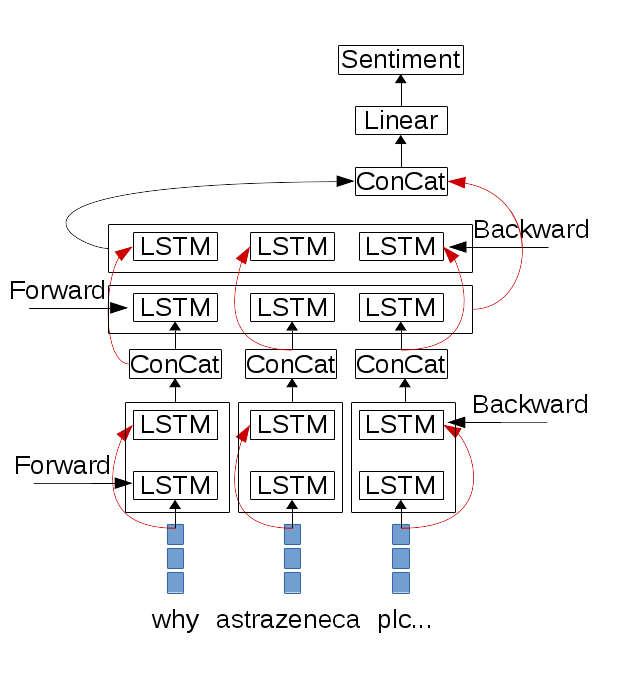
\includegraphics[scale=0.3]{lstm_diagram.png}

    \column{0.4\textwidth}

      \begin{block}{Standard Model (SLSTM)}
\begin{itemize}
\item Drop out between layers and connections.
\item 25 times trained over the data (epoch of 25).
\end{itemize}

\end{block}
\begin{block}{Early stopping model (ELSTM)}
\begin{itemize}
\item Drop out between layers only.
\item Early stopping used to determine the epoch.
\end{itemize}

\end{block}

  \end{columns}


\end{frame}

% We used the MSE loss function as we are predicting real values.
\begin{frame}[fragile]{BLSTM loss function}
\begin{columns}[T,onlytextwidth]
\column{0.6\textwidth}
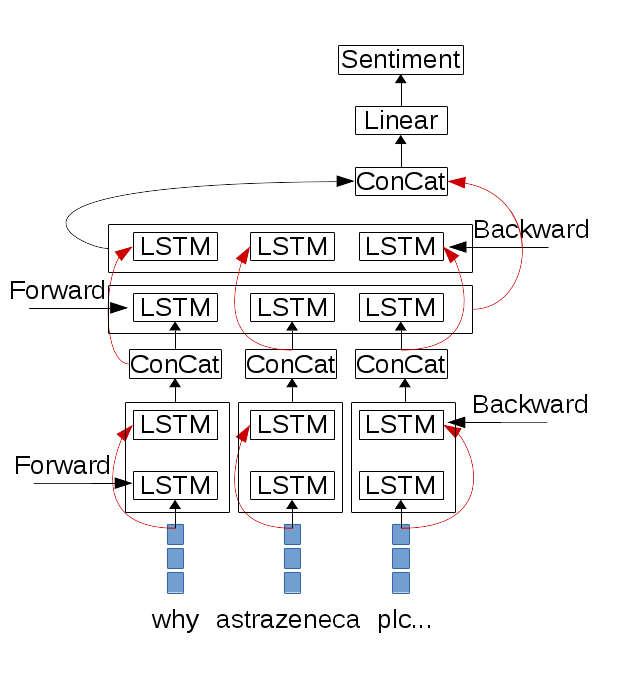
\includegraphics[scale=0.3]{lstm_diagram.png}

\column{0.4\textwidth}
\centering
\begin{block}{Loss function\newline Mean Square Error (MSE)}
\begin{equation}
\frac{1}{Y}\sum\limits_{i=1}^{Y} (\hat y_i - y)^2
\end{equation}

\end{block}
\end{columns}
\end{frame}




\section{Findings and Results}

\begin{frame}[fragile]{SVR best features}
\begin{block}{Features}
\begin{itemize}
\item Using uni-grams and bi-grams to be the best. 2.4\% improvement over uni-grams.
\item Using a tokeniser always better. Affects bi-gram results the most. 1\% improvement using Unitok\footnote{\url{http://corpus.tools/wiki/Unitok}} over whitespace.
\item SVR parameter settings important 8\% difference between using C=0.1 and C=0.01. 
\item Incorporating the target aspect increased performance. 0.3\% improvement.
\item Using all word replacements. N=10 for POS and NEG words and N=0 for company. 0.8\% improvement using company and 0.2\% for POS and NEG.
\end{itemize}
\end{block}

\end{frame}

\begin{frame}[fragile]{The three different metrics}

\begin{columns}[T,onlytextwidth]

\column{0.33\textwidth}
\begin{block}{Cosine Similarity (CS) Metric 1}
\begin{equation}
\frac{ \sum\limits_{i=1}^{K}{y_i  \hat y_i} }{ \sqrt{\sum\limits_{i=1}^{K}{y_i^2}}  \sqrt{\sum\limits_{i=1}^{K}{\hat y_i^2}} }
\end{equation}
\end{block}

\column{0.66\textwidth}
\begin{block}{Metric 2}
\begin{equation}
\label{eq:first_eval}
\begin{gathered}
\frac{\sum_{n=1}^{N} \text{CS}(\hat y_n, y_n)}{N}
\end{gathered}
\end{equation}
\end{block}

\begin{block}{Metric 3}
\begin{equation}
\begin{gathered}
\frac{\sum_{n=1}^{N} \begin{cases}len(\hat y_n) * \text{CS}(\hat y_n, y_n), & \text{if}\ len(\hat y_n) > 1 \\
      1 - \lvert y - \hat y_n \rvert, & \text{if}\ \frac{\hat y_n}{y}\geq0
      \end{cases} }{K}
\end{gathered}
\end{equation}

\end{block}

\end{columns}
\textit{K} = Total number of samples. \newline
\textit{N} = Total number of sentences.


\end{frame}

\begin{frame}[fragile]{Results across the different metrics}
\begin{table}[c]
\centering
\begin{tabular}{cccc}
 \multicolumn{1}{c}{} & \multicolumn{3}{c}{Metric} \\
 Model&  1&  2&  3 \\
 SVR&  62.14&  54.59&  62.34 \\
 SLSTM&  72.89&  61.55&  68.64 \\
 ELSTM&  73.20&  61.98&  69.24 \\
 Fortia-FBK\cite{Youness17}&  74.50&  -&  -
 
\end{tabular}
\end{table}

Metric 1 was the final metric used.
\end{frame}
\begin{frame}[fragile]{Error Analysis}
\centering
`uk stocks little changed as ashtead gains, housing shares drop'\\
Predicted: \textcolor{red}{-0.43}, Real: \textcolor{green}{0.23}

`standard life chief agrees £600000 bonus cut'\\
Predicted: \textcolor{red}{-0.54}, Real: \textcolor{green}{0.08}

`why i would put j sainsbury plc in my trolley before wm morrison supermarkets ...'\\
Predicted: \textcolor{green}{0.11}, Real: \textcolor{green}{0.76}

\end{frame}



\section{Future Work}

\begin{frame}[fragile]{Future Work}
\centering
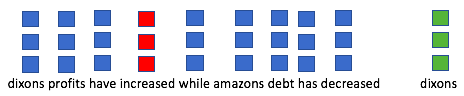
\includegraphics[scale=0.5]{sentence_attention.png}

\begin{enumerate}
\item Incorporate aspects into the BLSTM's shown to be useful by Wang et al. \cite{wangattention}.
\item Improve BLSTM's by using an attention model Wang et al. \cite{wangattention}.
\item Add known financial sentiment lexicon into the LSTM model \cite{Qian2017}.
\end{enumerate}

\end{frame}


\begin{frame}[fragile]{Summary}
\begin{enumerate}
\item BLSTM outperform SVRs with minimal feature engineering.
\item The future is to incorporate more financial information into the LSTM's.
\end{enumerate}

\end{frame}

\begin{frame}[plain]
\begin{center}
\begin{center}
\huge Questions?
\end{center}
\begin{center}
\begin{columns}[T,onlytextwidth]
\column{0.1\textwidth}
\column{0.4\textwidth}
\centering
\normalsize a.moore@lancaster.ac.uk
\normalsize p.rayson@lancaster.ac.uk
\column{0.4\textwidth}
\centering
\normalsize @apmoore94\\
\normalsize @perayson
\column{0.1\textwidth}
\end{columns}
\end{center}
\end{center}

\begin{center}
\begin{center}
\small All the code can be found here\footnote{\url{https://github.com/apmoore1/semeval}}
\end{center}
\begin{center}
\small Presentation can be found here \footnote{\url{https://github.com/apmoore1/semeval/blob/master/presentation/semeval.pdf}}
\end{center}
\end{center}

\end{frame}




\begin{frame}[allowframebreaks]{References}
  \bibliography{demo}
  \bibliographystyle{abbrv}

\end{frame}

\end{document}
